% GNUPLOT: LaTeX picture with Postscript
\begingroup
  \makeatletter
  \providecommand\color[2][]{%
    \GenericError{(gnuplot) \space\space\space\@spaces}{%
      Package color not loaded in conjunction with
      terminal option `colourtext'%
    }{See the gnuplot documentation for explanation.%
    }{Either use 'blacktext' in gnuplot or load the package
      color.sty in LaTeX.}%
    \renewcommand\color[2][]{}%
  }%
  \providecommand\includegraphics[2][]{%
    \GenericError{(gnuplot) \space\space\space\@spaces}{%
      Package graphicx or graphics not loaded%
    }{See the gnuplot documentation for explanation.%
    }{The gnuplot epslatex terminal needs graphicx.sty or graphics.sty.}%
    \renewcommand\includegraphics[2][]{}%
  }%
  \providecommand\rotatebox[2]{#2}%
  \@ifundefined{ifGPcolor}{%
    \newif\ifGPcolor
    \GPcolorfalse
  }{}%
  \@ifundefined{ifGPblacktext}{%
    \newif\ifGPblacktext
    \GPblacktexttrue
  }{}%
  % define a \g@addto@macro without @ in the name:
  \let\gplgaddtomacro\g@addto@macro
  % define empty templates for all commands taking text:
  \gdef\gplbacktext{}%
  \gdef\gplfronttext{}%
  \makeatother
  \ifGPblacktext
    % no textcolor at all
    \def\colorrgb#1{}%
    \def\colorgray#1{}%
  \else
    % gray or color?
    \ifGPcolor
      \def\colorrgb#1{\color[rgb]{#1}}%
      \def\colorgray#1{\color[gray]{#1}}%
      \expandafter\def\csname LTw\endcsname{\color{white}}%
      \expandafter\def\csname LTb\endcsname{\color{black}}%
      \expandafter\def\csname LTa\endcsname{\color{black}}%
      \expandafter\def\csname LT0\endcsname{\color[rgb]{1,0,0}}%
      \expandafter\def\csname LT1\endcsname{\color[rgb]{0,1,0}}%
      \expandafter\def\csname LT2\endcsname{\color[rgb]{0,0,1}}%
      \expandafter\def\csname LT3\endcsname{\color[rgb]{1,0,1}}%
      \expandafter\def\csname LT4\endcsname{\color[rgb]{0,1,1}}%
      \expandafter\def\csname LT5\endcsname{\color[rgb]{1,1,0}}%
      \expandafter\def\csname LT6\endcsname{\color[rgb]{0,0,0}}%
      \expandafter\def\csname LT7\endcsname{\color[rgb]{1,0.3,0}}%
      \expandafter\def\csname LT8\endcsname{\color[rgb]{0.5,0.5,0.5}}%
    \else
      % gray
      \def\colorrgb#1{\color{black}}%
      \def\colorgray#1{\color[gray]{#1}}%
      \expandafter\def\csname LTw\endcsname{\color{white}}%
      \expandafter\def\csname LTb\endcsname{\color{black}}%
      \expandafter\def\csname LTa\endcsname{\color{black}}%
      \expandafter\def\csname LT0\endcsname{\color{black}}%
      \expandafter\def\csname LT1\endcsname{\color{black}}%
      \expandafter\def\csname LT2\endcsname{\color{black}}%
      \expandafter\def\csname LT3\endcsname{\color{black}}%
      \expandafter\def\csname LT4\endcsname{\color{black}}%
      \expandafter\def\csname LT5\endcsname{\color{black}}%
      \expandafter\def\csname LT6\endcsname{\color{black}}%
      \expandafter\def\csname LT7\endcsname{\color{black}}%
      \expandafter\def\csname LT8\endcsname{\color{black}}%
    \fi
  \fi
  \setlength{\unitlength}{0.0500bp}%
  \begin{picture}(9636.00,5418.00)%
    \gplgaddtomacro\gplbacktext{%
      \csname LTb\endcsname%
      \put(814,704){\makebox(0,0)[r]{\strut{} 0}}%
      \csname LTb\endcsname%
      \put(814,1154){\makebox(0,0)[r]{\strut{} 10}}%
      \csname LTb\endcsname%
      \put(814,1605){\makebox(0,0)[r]{\strut{} 20}}%
      \csname LTb\endcsname%
      \put(814,2055){\makebox(0,0)[r]{\strut{} 30}}%
      \csname LTb\endcsname%
      \put(814,2505){\makebox(0,0)[r]{\strut{} 40}}%
      \csname LTb\endcsname%
      \put(814,2956){\makebox(0,0)[r]{\strut{} 50}}%
      \csname LTb\endcsname%
      \put(814,3406){\makebox(0,0)[r]{\strut{} 60}}%
      \csname LTb\endcsname%
      \put(814,3856){\makebox(0,0)[r]{\strut{} 70}}%
      \csname LTb\endcsname%
      \put(814,4307){\makebox(0,0)[r]{\strut{} 80}}%
      \csname LTb\endcsname%
      \put(814,4757){\makebox(0,0)[r]{\strut{} 90}}%
      \csname LTb\endcsname%
      \put(946,484){\makebox(0,0){\strut{} 1950}}%
      \csname LTb\endcsname%
      \put(2131,484){\makebox(0,0){\strut{} 1960}}%
      \csname LTb\endcsname%
      \put(3315,484){\makebox(0,0){\strut{} 1970}}%
      \csname LTb\endcsname%
      \put(4500,484){\makebox(0,0){\strut{} 1980}}%
      \csname LTb\endcsname%
      \put(5685,484){\makebox(0,0){\strut{} 1990}}%
      \csname LTb\endcsname%
      \put(6870,484){\makebox(0,0){\strut{} 2000}}%
      \csname LTb\endcsname%
      \put(8054,484){\makebox(0,0){\strut{} 2010}}%
      \csname LTb\endcsname%
      \put(9239,484){\makebox(0,0){\strut{} 2020}}%
      \put(176,2730){\rotatebox{-270}{\makebox(0,0){\strut{}Electricity in Millions of Tonnes of Oil Equivalent}}}%
      \put(5092,154){\makebox(0,0){\strut{}Year}}%
      \put(5092,5087){\makebox(0,0){\strut{}Electricity Demand UK: 1956-2013}}%
    }%
    \gplgaddtomacro\gplfronttext{%
      \csname LTb\endcsname%
      \put(8252,4584){\makebox(0,0)[r]{\strut{}Total}}%
      \csname LTb\endcsname%
      \put(8252,4364){\makebox(0,0)[r]{\strut{}Coal}}%
      \csname LTb\endcsname%
      \put(8252,4144){\makebox(0,0)[r]{\strut{}Oil}}%
      \csname LTb\endcsname%
      \put(8252,3924){\makebox(0,0)[r]{\strut{}Natural Gas}}%
      \csname LTb\endcsname%
      \put(8252,3704){\makebox(0,0)[r]{\strut{}Nuclear}}%
      \csname LTb\endcsname%
      \put(8252,3484){\makebox(0,0)[r]{\strut{}Natural Flow Hydro}}%
      \csname LTb\endcsname%
      \put(8252,3264){\makebox(0,0)[r]{\strut{}Wind}}%
      \csname LTb\endcsname%
      \put(8252,3044){\makebox(0,0)[r]{\strut{}Coke and Breeze}}%
      \csname LTb\endcsname%
      \put(8252,2824){\makebox(0,0)[r]{\strut{}Other Power}}%
    }%
    \gplbacktext
    \put(0,0){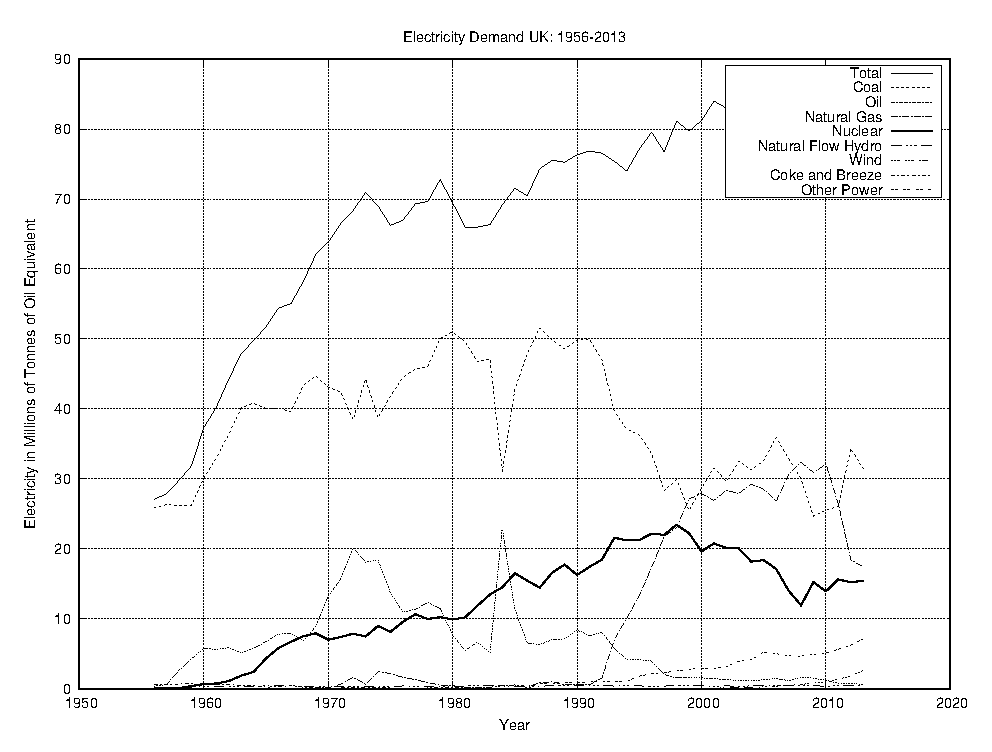
\includegraphics{chapter1/elec_demand}}%
    \gplfronttext
  \end{picture}%
\endgroup
